
% The \phantomsection command is needed to create a link to a place in the document that is not a
% figure, equation, table, section, subsection, chapter, etc.
% https://tex.stackexchange.com/questions/44088/when-do-i-need-to-invoke-phantomsection
\phantomsection

% Multiple-language document - babel - selectlanguage vs begin/end{otherlanguage}
% https://tex.stackexchange.com/questions/36526/multiple-language-document-babel-selectlanguage-vs-begin-endotherlanguage
\begin{otherlanguage*}{english}

% The \phantomsection command is needed to create a link to a place in the document that is not a
% figure, equation, table, section, subsection, chapter, etc.
% https://tex.stackexchange.com/questions/44088/when-do-i-need-to-invoke-phantomsection
\phantomsection

% Multiple-language document - babel - selectlanguage vs begin/end{otherlanguage}
% https://tex.stackexchange.com/questions/36526/multiple-language-document-babel-selectlanguage-vs-begin-endotherlanguage
\begin{otherlanguage*}{portuguese}

\chapter{\lang{Service Implementation}{Implementação do Serviço}} \label{cap:implementacao:servico}

Neste capítulo iremos trazer a experiência de implementação do Serviço para duas
diferentes implantações a primeira com CRIU e cri-o, que não conseguimos finalizar,
mas que possui importantes experiências e resolução de problemas a serem relatadas, e,
a segunda sendo a implantação utilizando técnicas de \textit{Event Sourcing} que foi
finalizada. Antes de apresentar as duas implementações iremos continuar apresentando
mais aplicações, bibliotecas e plataformas que utilizamos durante a implementação do
Serviço.

\section{Aplicações, bibliotecas e plataformas}

Para a implementação tanto do \textit{Checkpoint/Restore} com CRIU quanto com técnicas
de \textit{Event Sourcing} foi necessário a utilização de aplicações, bibliotecas e
plataformas que facilitaram o nosso desenvolvimento.

Um dos pontos iniciais para a implementação é o local para realizar a implantação do
Serviço. Inicialmente escolhemos utilizar a plataforma Emulab \cite{White+:osdi02}
que fornece máquinas virtuais sob demanda para computação distribuída. Embora, tudo
tenha funcionado bem com estas máquinas inicialmente, houveram dificuldades para
fazer funcionar o CRIU juntamente com o Kubernetes nas máquinas. Então, optamos por
trocar para outra solução mais comercial, o Google Cloud, nesta plataforma obtemos
uma máquina virtual permanente, desta forma, não era necessário refazer a configuração
da máquina todas as vezes. De modo, a economizar nos custos dos recursos de nossos testes,
eles foram feitos sob uma implantação em \textit{cluster} Kubernetes de máquinas com 2vCPU e 4GB
de memória, que é suficiente para executar um \textit{cluster} de nó único com Kubernetes.

Para possibilitar a existência da aplicação no Kubernetes nós precisamos adequar a
aplicação no fluxo de reconciliação de estado do Kubernetes através do conceito do Operador
\cite{kubernetes:operator}. Para isto, criamos três controladores, que são específicos para
cada recurso do Kubernetes e realizam o fluxo de reconciliação para os recursos, que juntos
implementam partes dos componentes da nossa arquitetura. O Interceptador é o único que não
foi implementado a através de um controlador. Teremos o controlador de Deployment, que é
responsável por verificar novos Deployments com anotação de monitoramento
\texttt{crsc.io/checkpoint-restore: true}, que indica que deve ser monitorado para
recuperação pelo Serviço, este controlador adiciona no Deployment o Interceptador como
um \textit{sidecar container}, que permitirá interceptar as requisições à aplicação alvo.
O controlador de Pod, será o responsável por monitorar os Pods e verificar quando houver a
anotação \texttt{crsc.io/checkpoint-restore: true} e o contêiner alvo da aplicação sofrer
uma falha, ou seja, não estiver no estado de Pronto do Kubernetes, ele ser agendado para
uma recuperação. Por fim, temos um outro controlador não totalmente
implementado, ele é o responsável por verificar o intervalo de \textit{Checkpoint} da
aplicação através da anotação do Deployment \texttt{crsc.io/checkpoint-interval}, sempre
que um novo Deployment monitorado for identificado, um recurso de Checkpoint é criado, e este
é monitorado pelo controlador do Checkpoint, quando se dá o momento do \textit{Checkpoint}
o controlador se comunica com o Interceptador e depois cria uma nova imagem a partir do
resultado do salvamento de estado do interceptador. Iremos cobrir com mais ênfase cada um
deles nas seções posteriores. Para construir todos este Operador, utilizamos o \textit{framework}
operator-sdk, que permite realizar a criação de recursos de Kubernetes e dos controladores
de maneira ágil e simples, abstraindo as intereções com o kube-apiserver e criação dos
Custom Resource Definition, que foram necessários para o novo recurso Checkpoint.

Ainda no contexto do \textit{Checkpoint}, como comentamos no capítulo de trabalhos
relacionados em \cite{schmidttransparent}, podemos obter um \textit{Checkpoint} da
aplicação utilizando o kubelet e as funcionalidades já implementadas para o cri-o
através da API do Kubernetes \cite{kubernetes:container-checkpoint}. Entretanto,
isso não nos gera uma imagem no formato do Open Container Initiative, devemos criar
essa imagem a partir de todos os passos que fizeram no trabalho em
\cite{schmidttransparent}. O caminho que optamos por seguir é um pouco diferente e
apresenta uma facilidade maior, na implementação de \cite{schmidttransparent} temos
o problema de dar manutenção na geração da imagem sempre que uma mudança na interface
ocorrer. Por isso, optamos por utilizar uma biblioteca e aplicação que já fizesse esta
parte a abstraisse o trabalho para nós, a biblioteca que encontramos, que também
funciona como uma aplicação de linha de comando, é o buildah\cite{buildah}. O buildah é
uma ferramenta especializada para facilitar a criação de imagens de contêineres no formato
do OCI.

Para armazenamento persistente dos dados da aplicação, como as requisições, utilizamos
o PostgreSQL \cite{postgresql} como banco de dados persistente. Ele será utilizado para
armazenar as requisições persistentemente quando necessário. Entretanto, a aplicação
pode funcionar utilizando memória, mas, esta implementação de memória existe problemas
dependendo da quantidade de memória livre para aplicação.

\section{Configuração do Cluster}

Para realizar a configuração do \textit{cluster} Kubernetes foram necessário realizar
algumas configurações e instalação de pacotes que fizessem CRIU, Kubernetes e buildah
funcionarem. Para configurar um \textit{cluster} Kubernetes com todas as funcionalidades
necessárias utilizamos Ubuntu 20.04, em máquinas com processador Intel Broadwell de
arquitetura x86/64 com 2vCPU e 4GB de memória, a partir disso precisamos executar a
sequência de comandos no Código \ref{listing:setup-script}, neste código utilizamos
o cri-o na versão 1.25, que é a versão necessária para fornecer suporte para CRIU no
\textit{Checkpoint} com o Kubernetes.

\begin{lstlisting}[language=bash,caption={Comandos de configuração da máquina para CRIU e cri-o.},label={listing:setup-script}]
   sudo sh -c 'echo "deb https://download.opensuse.org/repositories/devel:/kubic:/libcontainers:/stable/xUbuntu_20.04/ /" > /etc/apt/sources.list.d/devel:kubic:libcontainers:stable.list'
	sudo sh -c 'echo "deb http://download.opensuse.org/repositories/devel:/kubic:/libcontainers:/stable:/cri-o:/1.25/xUbuntu_20.04/ /" > /etc/apt/sources.list.d/devel:kubic:libcontainers:stable:cri-o:$CRIO_VERSION.list'
	curl -L https://download.opensuse.org/repositories/devel:/kubic:/libcontainers:/stable:/cri-o:/1.25/xUbuntu_20.04/Release.key | sudo apt-key add -
	curl -L https://download.opensuse.org/repositories/devel:/kubic:/libcontainers:/stable/xUbuntu_20.04/Release.key | sudo apt-key add -
	sudo apt-get update
	sudo apt-get install -y criu cri-o cri-o-runc
\end{lstlisting}

Primeiro adicionamos os repositórios para instalação do cri-o, que será utilizado como
\textit{runtime} de contêineres para o Kubernetes, e instalação dele, no mesmo comando
de instalação, instalamos o pacote do CRIU. No Código \ref{listing:setup-script} também
instalamos o \textit{backend} que o cri-o utiliza para contêineres, o runc, uma versão
específica deve ser instalada para que funcione o cri-o no Kubernetes.

Após instalado cri-o e CRIU, alteramos as configurações de ambos para que pudessemos
realizar o \textit{Checkpoint}. Primeiro, no Código \ref{listing:crio-conf}, alteramos
o comportamento da \textit{runtime} adicionando a opção que ativa o suporte para o CRIU
no cri-o e uma opção que remove a infraestrutura quando um contêiner não possui uma id de
processo privada, este deve ser ativado para mitigar um erro no cri-o. Estas alterações
foram feitas no arquivo /etc/crio/crio.conf.

\begin{lstlisting}[language=plaintext,caption={Configuração a ser incluída no arquivo de configurações do cri-o.},label={listing:crio-conf}]
[crio.runtime]
enable_criu_support = true # permite suporte a CRIU
drop_infra_ctr = false # remove a infra quando um pod não tem uma id de processo privada
\end{lstlisting}

Para que o CRIU possa utilizar o runc corretamente, também devemos editar a configuração
do CRIU. No Código \ref{listing:runc-conf}, editamos o arquivo /etc/criu/runc.conf para 
incluir configurações para fechar as conexões TCP, para ignorar conexões TCP já feitas,
onde o cliente deverá refazer as requisições, e desativamos a adiministração e cgroups
feita pela CRIU para utilizar o padrão.

\begin{lstlisting}[language=plaintext,caption={Configuração a ser incluída no arquivo de configurações do runc para o CRIU.},label={listing:runc-conf}]
tcp-close # fecha as conexões TCP
skip-in-flight # ignora conexões já abertas que devem ser refeitas depois do checkpoint
manage-cgroups=ignore
\end{lstlisting}

A próxima parte requer que tenhamos buildah instalado e o componentes principais do nó
mestre do Kubernetes, o kubeadm e o kubelet, como também o kubectl para acessar o cluster
através da  API do Kubernetes. Os comandos para instalação destes pacotes e componentes podem
ser instalados através do Código \ref{listing:kubernetes-setup}. O comando \texttt{sudo apt-mark hold}
é necessário para fixar as versões de instalação dos componentes do Kubernetes nas suas
versões em caso de atualização do sistema.

\begin{lstlisting}[language=bash,caption={Instalação dos pacotes necessários para Kubernetes e buildah.},label={listing:kubernetes-setup}]
sudo apt-get install -y apt-transport-https ca-certificates curl buildah make
sudo mkdir /etc/apt/keyrings
sudo sh -c "curl -fsSL https://pkgs.k8s.io/core:/stable:/v1.25/deb/Release.key | gpg --dearmor -o /etc/apt/keyrings/kubernetes-apt-keyring.gpg"
sudo sh -c 'echo "deb [signed-by=/etc/apt/keyrings/kubernetes-apt-keyring.gpg] https://pkgs.k8s.io/core:/stable:/v1.25/deb/ /" | tee /etc/apt/sources.list.d/kubernetes.list'
sudo apt-get update
sudo apt-get install -y kubelet kubeadm kubectl
sudo apt-mark hold kubelet kubeadm kubectl
\end{lstlisting}

Como o \text{Checkpoint} para contêineres no Kubernetes ainda é uma funcionalidade em alfa para
o Kubernetes, ela não é ativada automaticamente para toda nova instância de \textit{cluster}
Kubernetes. Precisamos alterar o funcionamento do Kubernetes para utilizar especificamente essa
funcionalidade, para isso existem os chamados \textit{Feature Gates} do Kubernetes que permitem
nas versões mais novas do Kubernetes ativar funcionalidades ainda não lançadas. Para ativar a
funcionalidade de \textit{Container Checkpoint} devemos alterar o arquivo de configuração que
determina a execução do kubelet no systemd do Ubuntu, em
/usr/lib/systemd/system/kubelet.service.d/10-kubeadm.conf, este arquivo deve estar como no
Código \ref{listing:kubelet-conf}. A parte que ativa o \textit{Feature Gate} é
\texttt{Environment="KUBELET\_FEATURE\_GATES\_ARGS=--feature-gates=ContainerCheckpoint=true"}. Já
a parte \texttt{Environment="KUBELET\_EXTRA\_ARGS=--cgroup-driver=systemd"} configura o kubelet
para utilizar o cgroup systemd para executar, isto coloca o cri-o no mesmo cgroup do kubelet, 
que permite que o último utilize o primeiro, caso isso não seja feito o kubelet não teria acesso
ao cri-o.

\begin{lstlisting}[language=plaintext,caption={Configuração do kubelet para executar no systemd com Feature Flag de ContainerCheckpoint e cgroup do systemd.},label={listing:kubelet-conf}]
[Service]
Environment="KUBELET_KUBECONFIG_ARGS=--bootstrap-kubeconfig=/etc/kubernetes/bootstrap-kubelet.conf --kubeconfig=/etc/kubernetes/kubelet.conf"
Environment="KUBELET_CONFIG_ARGS=--config=/var/lib/kubelet/config.yaml"
Environment="KUBELET_EXTRA_ARGS=--cgroup-driver=systemd"
Environment="KUBELET_FEATURE_GATES_ARGS=--feature-gates=ContainerCheckpoint=true"
# This is a file that "kubeadm init" and "kubeadm join" generates at runtime, populating the KUBELET_KUBEADM_ARGS variable dynamically
EnvironmentFile=-/var/lib/kubelet/kubeadm-flags.env
# This is a file that the user can use for overrides of the kubelet args as a last resort. Preferably, the user should use
# the .NodeRegistration.KubeletExtraArgs object in the configuration files instead. KUBELET_EXTRA_ARGS should be sourced from this file.
EnvironmentFile=-/etc/default/kubelet
ExecStart=
ExecStart=/usr/bin/kubelet $KUBELET_KUBECONFIG_ARGS $KUBELET_CONFIG_ARGS $KUBELET_KUBEADM_ARGS $KUBELET_EXTRA_ARGS $KUBELET_FEATURE_GATES_ARGS
\end{lstlisting}

Por fim, iniciamos o \textit{cluster} Kubernetes através dos comando no Código
\ref{listing:kubernetes-conf}, desativamos o swap da máquina para não criar conflitos que podem
ocorrer no kubelet. Outra seção do Código \ref{listing:kubernetes-conf} é a configuração do
KUBECONFIG, que é a configuração que o kubectl utiliza para se comunicar com a API do Kubernetes.
Ao final do listing nós adicionamos um controlador de rede para os Pods do nosso sistema, qualquer
um pode ser utilizado, mas optamos por utilizar o Calico \cite{calico} pela facilidade em
instalação como vista na seção do Código \ref{listing:kubernetes-conf}

\begin{lstlisting}[language=bash,caption={Inicialização do Kubernetes, configuração de acesso para o kubectl e instalação do administrador de rede para Pods Calico.},label={listing:kubernetes-conf}]
# Start Kubernetes

sudo swapoff -a
sudo kubeadm init --pod-network-cidr=192.168.0.0/16 --ignore-preflight-errors='all'

# Init kubectl

mkdir -p $HOME/.kube
sudo cp -i /etc/kubernetes/admin.conf $HOME/.kube/config
sudo chown $(id -u):$(id -g) $HOME/.kube/config

# Add network manager. We are going to install Calico.

kubectl create -f https://raw.githubusercontent.com/projectcalico/calico/v3.26.1/manifests/tigera-operator.yaml
kubectl create -f https://raw.githubusercontent.com/projectcalico/calico/v3.26.1/manifests/custom-resources.yaml
\end{lstlisting}

A partir das configurações listadas nesta seção obtivemos um \textit{cluster} Kubernetes funcional
pronto para iniciar nossas implementações, que permitem a utilização de CRIU para o \textit{Checkpoint}
e de buildah para construção das imagens de recuperação.

\section{Interceptador}

O nosso Interceptador como descrito nas seções anteriores é implantado a partir de um
\textit{sidecar container}, ambas as versões do Serviço, a de \textit{Checkpoint/Restore}
a partir do CRIU e a do \textit{Checkpoint/Restore} a partir de técnicas de
\textit{Event Sourcing} utilizam o mesmo Interceptador que é a funcionalidade comum aos
dois. Para criá-lo utilizamos a linguagem de programação Go e
realizamos uma construção de sua imagem utilizando Docker, não é necessário utilizar
cri-o para construir a imagem neste caso, pois as imagens geradas também seguem OCI.
A aplicação consiste de um servidor HTTP, este servidor possui algumas funcionalidades
expostas que serão chamadas de acordo com a necessidade dos outros componentes.
O Interceptador possui um estado interno que pode estar em dois valores diferentes,
ou em Ativo ou em Aguardo. No Ativo enviamos todas as requisições interceptadas a
aplicação alvo do Serviço, já no estado Aguardo nós realizamos o armazenamento das
requisições e esperamos o estado retornar a Ativo para continuar a entrega das
requisições. Enquanto seguimos o fluxo do diagrama da Figura
\ref{fig:interceptor-request-interception} para interceptação das requisições durante
o estado de Pronto do Interceptador, a Figura \ref{fig:diagram-wait-state-interceptor}
representa o fluxo de interceptação quando o estado do Interceptador é Aguardo.

\begin{figure}[h]
\centering
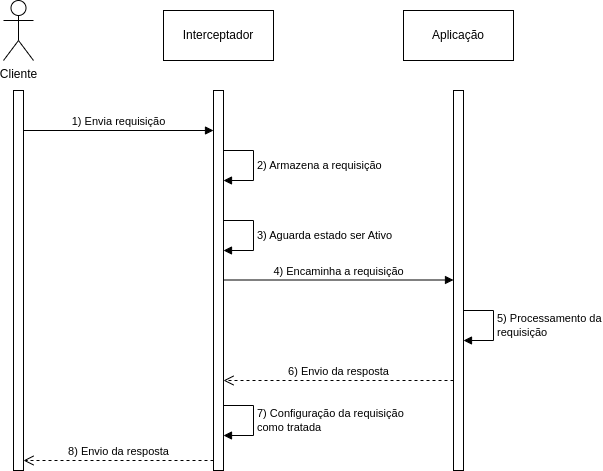
\includegraphics[scale=0.64]{images/wait-state.png}
\caption{Diagrama de sequência para tratamento de requisições durante estado de Aguardo do Interceptador.}
\label{fig:diagram-wait-state-interceptor}
\end{figure}

Para realizar um \textit{Checkpoint}, expomos uma rota HTTP de \texttt{/checkpoint}, que
chama a API do Kubernetes para que o kubelet comunique com o cri-o para realizar um 
\textit{Checkpoint} da aplicação executando no contêiner dentro do Pod alvo utilizando
CRIU. De modo a realizar a comunicação com o kube-apiserver precisamos estar autenticados
com o Kubernetes. Deste modo, criamos um Secret no Kubernetes, uma configuração de segredo
disponível na API do Kubernetes, com o certificado e key de assinatura para comunicação
com o kube-apiserver, estes arquivos ficam localizados no cluster em
/etc/kubernetes/pki/apiserver-kubelet-client.key e em
/etc/kubernetes/pki/apiserver-kubelet-client.crt, adicionamos estes dois arquivos em um
Secret como no Código \ref{listing:kubelet-secret}. Então, podemos chamarmos a API
do Kubernetes na rota <https://ip-do-cluster/checkpoint/namespace/pod/container>
utilizando o método HTTP POST, onde ip-do-cluster é o IP do \textit{cluster} Kubernetes,
é o \textit{namespace} do Kubernetes em que se encontra a aplicação do Kubernetes, pod é
o Pod que está executando a aplicação alvo e container o contêiner que está executando a
aplicação alvo. A partir daí, um \textit{Checkpoint} é salvo na máquina em
/var/lib/kubelet/checkpoints na forma de um arquivo compactado da forma
checkpoint-pod\_namespace-container-timestamp.tar, em que os valores são os mesmo,
exceto, \textit{timestamp}, que representa a string do momento em que o \textit{Checkpoint}
foi feito.

\begin{lstlisting}[language=bash,caption={Criação do Secret para comunicação com o kubelet para compartilhamento com nosso Interceptador.},label={listing:kubelet-secret}]
kubectl create secret generic kubelet-client-certs --from-file=client.crt=/etc/kubernetes/pki/apiserver-kubelet-client.crt --from-file=client.key=/etc/kubernetes/pki/apiserver-kubelet-client.key
\end{lstlisting}

Outra rota do Interceptador é a do estado em \texttt{/state}, através de uma chamada
HTTP ao método POST podemos alterar o estado com o parâmetro na \textit{query}
\texttt{state}, sendo ou Active, ou Waiting, que coloca o Interceptador nos estados,
respectivamente, de Ativou e Aguardo. O estado inicial do Interceptador é o Ativo.

Por fim, nós temos a rota \texttt{/reproject} que é a reprojeção de todas as requisições
interceptadas pelo Interceptador e aceita pela aplicação alvo. Esta reprojeção permite
que o estado seja alcançado. O ideal nesta reprojeção seria que ela pudesse ser feita a
partir de uma versão das requisições. Entretanto, não a fizemos porque não foi possível
finalizar a parte do \textit{Checkpoint/Restore} com CRIU que necessitaria desta parte.

\section{Checkpoint/Restore com CRIU}

Na implementação de \textit{Checkpoint/Restore} com CRIU criamos os três controladores do
nosso Operador, o controlador dos Deployments, o controlador dos Pods e o controlador do
nosso recurso customizado Checkpoint. Nesta implementação temos três passos para toda
aplicação monitorada, criação e implantação de um manifesto do Deployment da aplicação
no Kubernetes. Posterior criação do recurso customizado Checkpoint e monitoramento das
falhas do contêiner monitorado e posterior recuperação. Estes passos serão feitos pelos 
nossos controladores e descrevemos elas na próxima subseção.

\subsection{Controladores}

Todos os controladores do Kubernetes possuem um ciclo de reconciliação que deve
verificar o estado do \textit{cluster} e, em caso, de modificação do estado de algum
recurso que ele monitora deve agir de acordo com a alteração de estado para alcançar
um estado dos outros recursos de acordo com o que ele tem definido através dos manifestos
dos recursos.

\subsubsection{Controlador de Deployment}

O controlador do Deployment tem como seu recurso monitorado os Deployments do
\textit{cluster}. Sempre que uma aplicação é criada ela deve ser criada com anotações
no manifesto do Deploment, como \texttt{crsc.io/checkpoint-restore} e
\texttt{crsc.io/checkpoint-interval}, que são respectivamente, o valor booleano que
define se a aplicação é monitorada pelo Serviço ou não e o valor do intervalo de
\textit{Checkpoint} ativo. O diagram da Figura \ref{fig:deployment-controller-diagram}
define o funcionamento do controlador.

\begin{figure}[h]
\centering
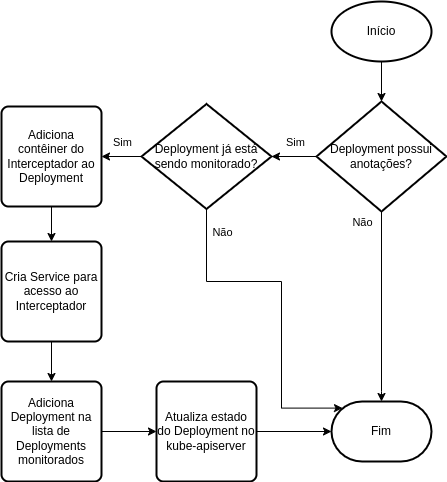
\includegraphics[scale=0.8]{images/deployment-controller.png}
\caption{Diagrama de fluxo para a injeção das configurações do Interceptador na aplicação alvo através de um Controlador de Deployments para o Operador.}
\label{fig:deployment-controller-diagram}
\end{figure}

A partir da alteração do estado do \textit{cluster} pela criação de um novo Deployment
monitorado o controlador realiza a criação de um novo recurso de Checkpoint. Este novo
recurso possui um manifesto com os valores de intervalo de \textit{Checkpoint} e também
as informações da aplicação monitorada, como o nome do Deployment. Este recurso será 
monitorado pelo controlador de Checkpoint que irá executar as ações necessárias para
alcançar o estado definido pelo manifesto.

Este controlador também deve injetar o Interceptador como um \textit{sidecar container}
ao Deployment da aplicação alvo. Sempre que um Deployment novo é adicionado com a 
anotação \texttt{crsc.io/checkpoint-restore} o manifesto do Deployment é alterado
para adicionar o contêiner do Interceptador como um \textit{sidecar container}, um novo
ReplicaSet é, então, criado pelo Kubernetes que criará um novo Pod com o nosso
Interceptador. Ao mesmo tempo o controlador cria um novo Service para o Interceptador no
novo Deployment que permite o Interceptador seja acessado através de todo o cluster, o
Kubernetes lida com a parte do DNS e das configurações de rede.

Ao final temos a adição no manifesto do Deployment do conteúdo do contêiner como visto no
Código \ref{listing:sidecar-container}. Este contêiner tem montado na imagem um volume
que indica os arquivos de assinatura na comunicação com o kube-apiserver que criamos na
Seção de configuração do \textit{cluster}. Isto permite que o nosso Interceptador possa
se comunicar de forma segura e autenticada com o Kubernetes para solicitar um novo
\textit{Checkpoint} ao kubelet.

\begin{lstlisting}[language=yaml,caption={Configuração do Interceptador para o Deployment da aplicação alvo como sidecar container.},label={listing:sidecar-container}]
image: docker.io/gianaortiz/crsc-interceptor
imagePullPolicy: Always
name: interceptor
ports:
- containerPort: 8001
  hostPort: 8001
  protocol: TCP
resources: {}
terminationMessagePath: /dev/termination-log
terminationMessagePolicy: File
volumeMounts:
- mountPath: /var/run/secrets/kubelet-certs
  name: kubelet-certs
  readOnly: true
\end{lstlisting}

A partir desse momento nossa aplicação monitorada tem suas requisições interceptadas
pelo nosso Interceptador. Inicialmente, o estado é Ativo no Interceptador, então todas
as requisições serão primeiro armazenadas e depois encaminhadas à aplicação para que
elas sejam tratadas.

\subsubsection{Controlador de Pod}

Para implementar o nosso Administrador de Estado, implementamos parte dele no controlador
de Pod. O controlador tem uma adiministração mais passiva, através do ciclo de
reconciliação, quando um Pod apresenta um problema, como por exemplo, um dos contêineres
falhar, o controlador filtra os Pods que possuem a anotação
\texttt{crsc.io/checkpoint-restore}, adicionando a uma fila de restauração.
A restauração aconteceria a partir da configuração de utilização de uma nova
imagem à aplicação monitorada, entretanto, não conseguimos criar a imagem de
\textit{Checkpoint} e esta parte não foi feita.

Na Figura \ref{fig:restore-pod} temos o diagrama de como funciona esta parte. Primeiro o
controlador recebe uma atualização de estado dos Pods, verificamos se o Pod é um Pod monitorado,
caso seja e tenha um contêiner com falha, iremos adicioná-lo à fila de restauração. Caso a
atualização de estado indique que ele está pronto iremos buscar o Pod na fila de restauração,
então, editaremos a imagem da aplicação alvo para que seja a imagem do último \textit{Checkpoint}
feito pelo controlador de Checkpoint. Após alterarmos a imagem, colocamos o Interceptador no
estado Aguardo e pedimos para ele reprojetar as requisições a partir da última requisição
recebida antes de se realizar o \textit{Checkpoint} atual. Ao final da reprojeção, alteramos
o estado do Interceptador para Ativo e as requisições são encaminhadas para a aplicação alvo
com o estado mais atual, fornecendo uma recuperação transparente ao usuário.

\begin{figure}[h!]
\centering
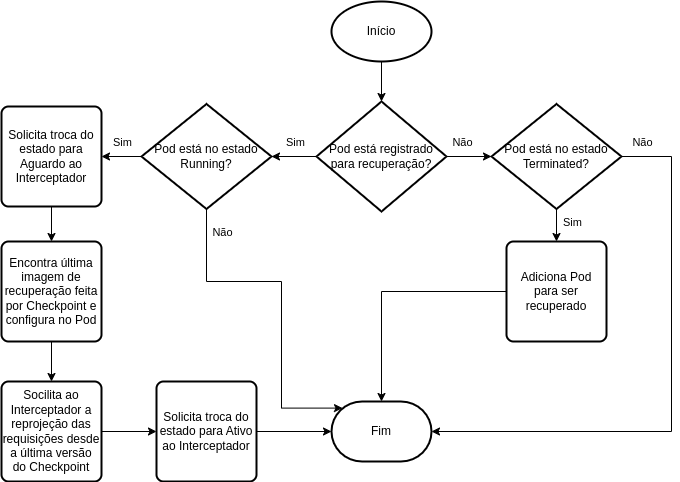
\includegraphics[scale=0.64]{images/restore-pod-criu.png}
\caption{Diagrama de fluxo para a recuperação da aplicação alvo através de um Controlador de Pods para o Operador com a implementação com CRIU.}
\label{fig:restore-pod}
\end{figure}

\subsubsection{Controlador de Checkpoint}

O controlador de Checkpoint realiza o ciclo de reconciliação para os recursos que nosso
Operador criou do tipo Checkpoint. O recurso Checkpoint possui o intervalo que é
passado através da anotação \texttt{crsc.io/checkpoint-interval} e o nome do Deployment
que está sendo monitorado. Através dessa anotação nosso controlador cria um processo que
será executado no intervalo dado para pedir um \textit{Checkpoint} ao Interceptador da
aplicação ao chamar a rota \texttt{/checkpoint} no Service do Interceptador. O Interceptador
irá pedir um novo \textit{Checkpoint} a API do kubelet e retornar sucesso. Após o sucesso,
este controlador irá obter esse \textit{Checkpoint} e criará uma imagem de contêiner no
formato OCI com buildah.

Como o este controlador também implementa uma parte do nosso Administrador de Estado da 
arquitetura geral, ele também seria o responsável por salvar informações de metadados
sobre a imagem de salvamento criada. Entretanto, não foi possível criar uma aplicação
que conseguisse utilizar as bibliotecas do buildah para criação da imagem, muitos
problemas foram encontrados ao se utilizar overlayfs como comunicação de disco e não
houve tempo para realizar no nosso Serviço a geração da imagem. Porém, conseguimos criar
uma imagem com buildah através da sequência de comandos no Código
\ref{listing:buildah-build}, que podem ser refeitos através da biblioteca e agregados ao
Serviço.

\begin{lstlisting}[language=bash,caption={Comandos do buildah para construir a imagem de recuperação a partir de um Checkpoint feito pelo CRIU através do kubelet.},label={listing:buildah-build}]
newcontainer=$(buildah from scratch)
buildah add $newcontainer /var/lib/kubelet/checkpoints/checkpoint-<pod-name>_<namespace-name>-<container-name>-<timestamp>.tar /
buildah config --annotation=io.kubernetes.cri-o.annotations.checkpoint.name=<container-name> $newcontainer
buildah commit $newcontainer checkpoint-image:latest
buildah rm $newcontainer
\end{lstlisting}

Embora o \textit{Checkpoint} impeça as requisições de chegarem à aplicação alvo
diretamente, ele ocorre de forma transparente ao usuário da aplicação. Não é
necessário entender que ele está acontecendo e não se percebe a existência dele. 
Estes \textit{Checkpoints} periódicos seriam utilizados para recuperar a aplicação
ao último estado de forma mais rápida e eficiente como em \cite{vayghan2021kubernetes}
\cite{muller2022architecture} \cite{oh2018stateful} e \cite{schmidttransparent}.

\section{Checkpoint/Restore com técnicas de Event Sourcing}

Na nossa implementação a partir de técnicas de Event Sourcing tinhamos o objetivo de
prover uma forma de agilizar a restauração da aplicação sem o problema do tempo que leva
para realizar o \textit{Checkpoint} da imagem. Já esperávamos que a performance para
aplicações com muitas requisições fosse pior, pois, necessitariamos reenviar todas as
requisições desde o início do estado de Pronto da aplicação. Mas, a partir dela
poderíamos unir com a técnica de \textit{Checkpoint} com CRIU para realizar ou uma ou
outra dependendo do estado atual do sistema, eliminando o tempo gasto em um
\textit{Checkpoint} no começo do estado de vida da aplicação. Assim, teremos algumas
modificações para alguns controladores que mostramos na Seção passada, já que alguns
passos não são realizados para nossa implementação com técnicas de \textit{Event Sourcing}.

\subsection{Controladores}

\subsubsection{Controlador de Deployment}

O controlador de Deployment para a implementação com técnicas de \textit{Event Sourcing} é
a mesma que para a implementação com CRIU, exceto, que, não criamos o recurso de Checkpoint neste
caso, pois, não há necessidade. Devido ao fato de sempre estarmos salvando as requisições
interceptados pelo Interceptador, sempre temos a ordem de requisições que precisamos
executar para obter o mesmo estado na aplicação alvo. Não precisamos realizar um
\textit{Checkpoint} periódico como no outro caso, pois, o salvamento de estado esta nos
eventos que são gerados pelas requisições. Neste controlador, também adicionamos o 
\textit{sidecar container} ao Deployment e criamos o Service que redireciona requisições
ao Interceptador. O Interceptador tem sempre a mesma implementação, o que permite ser
utilizado em diferentes sistemas e diferentes contextos, já que tudo que ele provê é uma
API.

\subsubsection{Controlador de Pod}

O controlador de Pod para a implementação com técnicas de Event Sourcing funciona
diferente da implementação com CRIU. Pois, neste caso não precisamos alterar a imagem da
aplicação alvo, ela permanece a mesma sempre, tudo que precisamos realizar é a sequência
na Figura \ref{fig:pod-controller-event-sourcing}. Primeiro identificamos um contêiner
falhante a partir da atualização do kube-apiserver, adicionamos ele a uma fila de
restauração caso ele seja monitorado através das anotações. Posteriormente a isso, quando
o Pod atinge o estado de Pronto, recebemos mais uma atualização, caso o Pod esteja na
fila de recuperação o Interceptador será colocado no estado Aguardo, será solicitada a
reprojeção das requisições. Após o fim da reprojeção das requisições, que podem demorar,
já que devemos fazer todas desde o ínicio do funcionamento da aplicação alvo, alteramos
o estado do Interceptador para Pronto novamente. Novamente, de forma transparente
recuperamos o contêiner da aplicação alvo para um estado consistente.

\begin{figure}[h]
\centering
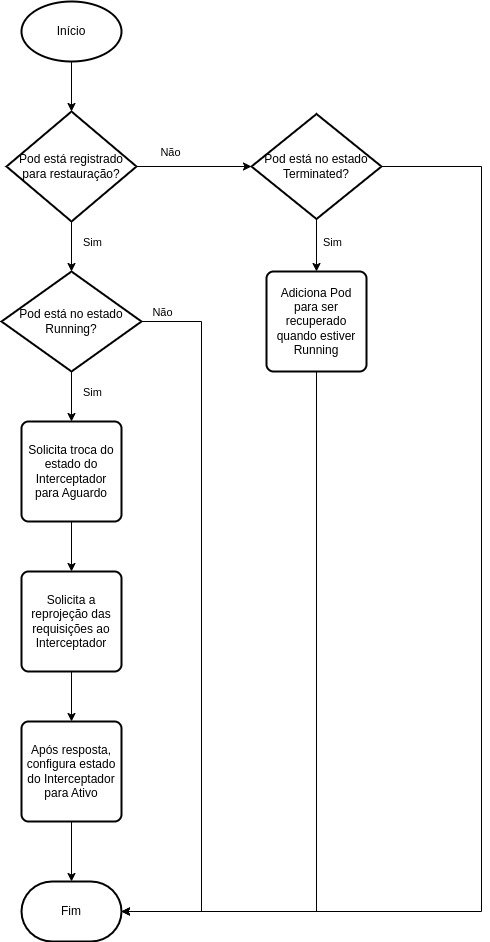
\includegraphics[scale=0.64]{images/restore-pod.png}
\caption{Diagrama de fluxo para a recuperação da aplicação alvo através de um Controlador de Pods para o Operador na implementação com técnicas de \textit{Event Sourcing}.}
\label{fig:pod-controller-event-sourcing}
\end{figure}

Desta forma, teriamos uma implementação que supostamente perderia performance dado
o número das requisições. Quanto mais requisições o sistema recebe, mais demorado seria
a reprojeção de todas as requisições, iremos validar este ponto na próxima Seção.
Entretanto, vale notar que esta é uma implementação não tão abordada em outros trabalhos,
exceto em \cite{muller2022architecture} que utiliza o conceito até certo ponto para
replicar as requisições a partir do último ponto de salvamento anterior a recuperação
da aplicação, o que diminui a latência em se recuperar a aplicação.

Como inicialmente pretendiamos adicionar as duas implementações, uma com CRIU e outra
com \textit{Event Sourcing}, pretendíamos aproveitar os pontos positivos de cada uma.
Entretanto, apenas a versão da implementação com técnicas de \textit{Event Sourcing}
foi finalizada e, pretendemos, na próxima Seção, investigar se essa implementação
realmente sofre de todas as partes negativas que apontamos nesta Seção.

\end{otherlanguage*}
